\subsection{Age structure and public transfers}
The immigrant and native populations are different not only in their size but also in their age structure.
By dividing total (across all ages) transfer by the total population, per-capita comparison between immigrant and natives account for the difference in the population size but not for the difference in age structure.
Public transfers are inter-generational; this implies collecting resources from the working-age population (t¢he outflow transfers) and reallocating them to the dependent population, mostly the young and old (the inflows transfers). Therefore, they are sensitive to the population's age structure.
Therefore the comparison based on per-capita values is biased because (to the same extent) the two populations have different age structures.
The decomposition discussed earlier is applied to the surpluses in each account and sub-account separately to account for this difference in age structure.
The decomposition function takes the age-specific transfer and the population size as inputs for a given transfer account. It then applies the decomposition algorithm and returns the two components representing the respective contributions of the inputs to the per crude surplus.
Doing so allows extracting the share of crude surplus accrued by a difference in age-specific transfer rather than a difference in the age structure of the two populations.

\vspace{0.7em}\par
Age-adjusted surpluses are the components associated with the age-specific transfers and represent the difference between an immigrant and a native of the same age.
We will also refer to these as fiscal components
On the other hand, demographic components are associated with the population size and represent the portion of the surplus that results from a difference in the age structure of immigrant and native populations.
As a reminder,
It is important to note that even though the population size is one of the inputs, the per-capita calculation cancels out any effect it may have had on the surpluses.
Also, as Net Surplus is the sum of all Immigrant Surpluses across all accounts (inflows minus outflow), the age-adjusted Net Surplus is computed similarly, as the sum of all age-adjusted Immigrant Surpluses. \autoref{fig:DEcomp} presents the trend in the crude and age-adjusted surpluses as well as the demographic components for each sub-accounts throughout the studied period.

\begin{figure}[H]%
  \caption{Trends in Crude, Age-adjusted and demographic components for accounts of inflows and outflows between 1997 and 2015 }
  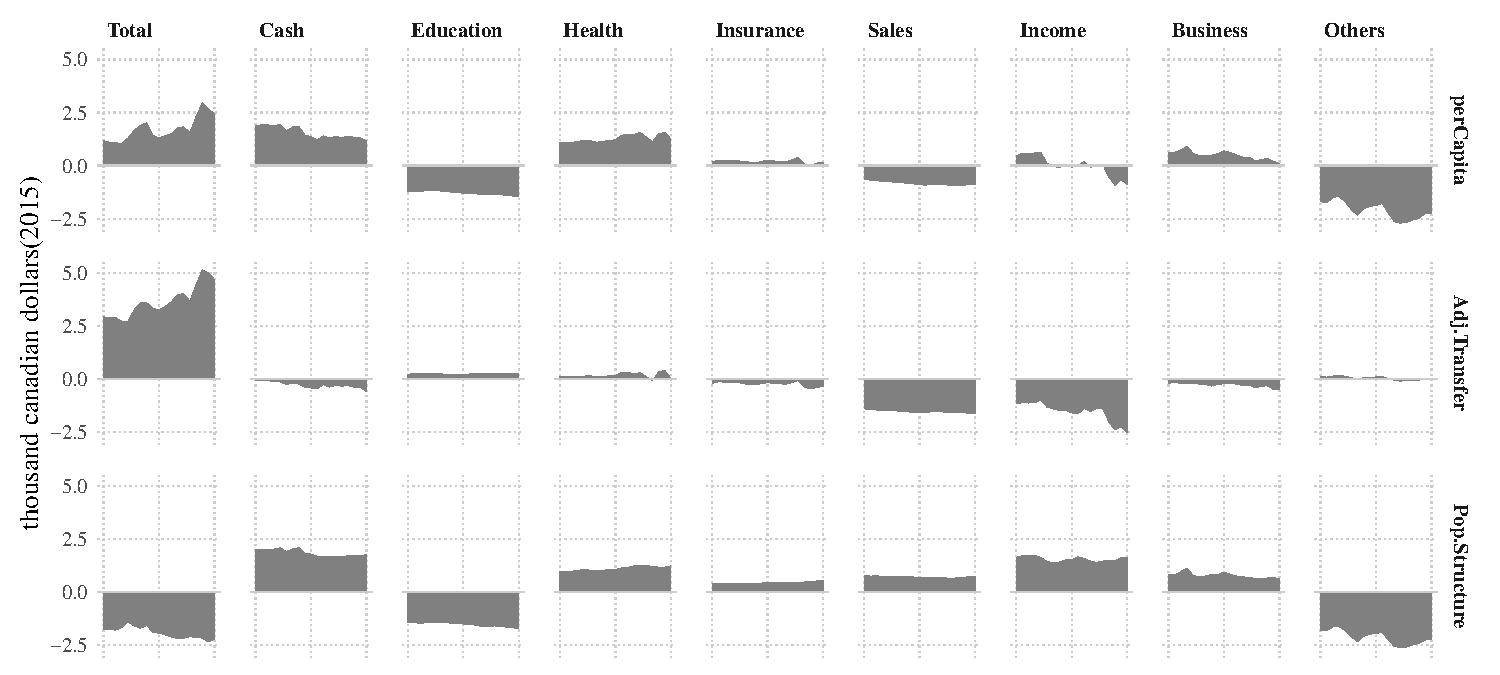
\includegraphics[width=1\textwidth]{../ntaImmig/res/DEcomp.pdf}%
  \label{fig:DEcomp}%
\end{figure}%

\subsection{Age-adjusted Net Surplus}

Results show that age-adjusted Net Surplus followed the same pattern as per-capita Net Surplus, but the levels are much higher in absolute values.
Furthermore, the overall negative sign for demographic components of Net Surplus indicates that age structure is much favourable to immigrants, as it reduced the difference between immigrants and natives from the adjusted value to the per-capita value.
In other words, the per-capita difference would have been much higher than its current (crude) value if the immigrant and native populations had the same age structure.
In dollar value, at equal age, the average immigrant has cost to the state about \DTLfetch{statex}{sKey}{AveAdj.Transfer}{sVal}\$ per year, more than the average native, between 1997 and 2016.
However, a favorable population structure reduced this surplus by about of \DTLfetch{statex}{sKey}{AvePop.Structure}{sVal}\$, leading the  \DTLfetch{statex}{sKey}{AveperCapita}{sVal}\$ in per-capita Net Surplus.
While the demographic effect has increased steadily during the studied period from \DTLfetch{statex}{sKey}{AvePop.Structure1997}{sVal}\$ to \DTLfetch{statex}{sKey}{AvePop.Structure2015}{sVal}\$, the trends in Adjusted Net Surplus are much stepping with disruptive increases every few years (early 2000, late 2000, early 2010) from \DTLfetch{statex}{sKey}{AveAdj.Transfer1997}{sVal}\$ in 1997 to \DTLfetch{statex}{sKey}{AveAdj.Transfer2015}{sVal}\$ in 2015.
The steady increase of the demographic components over the years reflects the faster ageing of the native population, as the immigrant population has been purposefully kept young through various economic immigration programs.

\vspace{0.7em}\par
These results imply that the difference in age structure between immigrant and native populations accounts for much of their difference in crude surpluses.
Therefore, not accounting for the demographic effect leads to conflicting results that confuse our understanding of transfer differential between immigrants and natives, create unnecessary discord in the immigration debates, and lead to inappropriate public policy.
The confusion goes even further when comparing the sub-account of inflow and outflow.

\subsection{Age-adjusted surpluses in sub accounts}

Looking at the adjusted surplus for the sub-accounts, it appears that income and sales taxes are the primary sources of the Net Surplus.
This result makes sense because the other sub-accounts tied to public programs are less likely to increase social inequality, such as the Immigrant Surplus.
On the other hand, the sub-accounts of Income and Sales taxes directly relate to individual revenue, which is more subjected to labour market outcome than public policy.
However, this pattern is not observable from the crude values, and crude Net Surplus shows opposite results, with inflows appearing as the primary sources of disparities in Net Transfers.
For example, most contributions to public finances represent a given proportion of the individual's income.
Therefore, it is intuitive that income taxes reflect the difference between immigrants and natives to a large extent.
On the contrary, the crude Net Surplus for income taxes shows conflicting results, positive between 1997 and 2003, null till 2012, and negative afterward.

\vspace{0.7em}\par
These results illustrate the mitigating effect of demographic components in the differences in transfer between immigrants and natives.
Demographic differences are also the reasons for the high per-capita health care cost, which reduced to close to zero in the age-adjusted surplus.
Therefore, the high difference in health care transfer between immigrants and natives implies that there are relatively more immigrants in the age groups with the highest health care costs.

\vspace{0.7em}\par
Demographic differences not only affect the size of the Immigrant Surplus but also change its direction and trend.
For example, looking at the per-capita surplus, immigrants seem to have paid on average more business taxes than natives.
The situation reverses after adjusting for demographic effects, with immigrants paying less in business taxes than natives. Moreover, the trend in Immigrant Surplus is increasing as opposed to the per-capita measure.
The low business taxes paid by immigrants suggest that they operate smaller businesses than natives.
They also contributed toward social security and received cash transfers, slightly less than natives.
The opposite applies to education and health care costs, where immigrants consume slightly more than natives.

\vspace{0.7em}\par
The Other sub-account of transfer include public goods and services as well as public deficits and debts.
By design, the NTA method distributes these costs evenly, making no difference between immigrants and natives.
As a result, the age-adjusted surplus for the other sub-accounts is close to zero and the lowest absolute value among all sub-accounts.
Therefore the significant negative effect (in favour of natives) seen in the per-capita surplus is mainly due to the difference in age structure between immigrants and natives.
When adjusted for these differences, the surpluses in these other sub-accounts compensated each other, revealing the sub-account of sales and income taxes as the two most important sources of disparities between immigrants and natives.

\vspace{0.7em}\par
In summary, immigrants received similar benefits from public programs, but their low revenue does not contribute equally to public finances, leading to a positive Net Surplus.
As a result, difference in sales and income taxes added up to an age-adjusted surplus of \DTLfetch{statex}{sKey}{SIAdjusted}{sVal}\$ which  represent \DTLfetch{statex}{sKey}{SIprop}{sVal}\% of the \DTLfetch{statex}{sKey}{AveAdj.Transfer}{sVal}\$ in total age-adjusted surplus.
As these taxes come from income mainly earned from labour, the labour market stands out as a significant source of inequality between immigrants and natives.
Furthermore, it appears that while both income and sales taxes are the main contributors to Net Surplus, income taxes alone drive its trends.
These results stand against the expectations of a positive impact of immigration on public finances, especially for recent immigrants for whom economic factors have motivated the admission.
Therefore understanding how the labour market has become the source of so many imbalances, especially since 2011, is a crucial question to discuss and address should Canada intend to benefit from its immigrants.


















